\section{Presentación}
Como se expuso en el capítulo anterior,  Carathéodory introdujo este principio como antesala de lo que la gente conocía como la primera ley de la termodinámica, que en esencia apela a la conservación de la energía para definir el concepto de calor. Otras formulaciones, modernas, presentan también cuatro principios, en donde el primer postulado (no lo llamaremos principio cero) propone la existencia de los estados de equilibrio, aún como la existencia de las variables macroscópicas tales como la energía interna, el volumen, y los números de moles de las especies químicas que conforman el sistema. La versión de Carathéodory propone en esencia que los estados de equilibrio entre sistemas térmicos forman clases de equivalencia, y deja los conceptos de variables macroscópicas, sistema y estado como conceptos primitivos.\\
El presente autor, considera también que los conceptos de sistema térmico, variable macroscópica, estado, equilibrio, región (del espacio), frontera e interacción entre sistemas, son conceptos primitivos, es decir, de entrada en la presente formulación de los principios básicos de la termodinámica. Sin embargo, los cuatros principios conceptos citados se introducen en la presente versión del principio cero de la termodinámica como una versión ampliada de la original propuesta por Carathéodory.\\

\begin{description}
\item[Principio Cero.] Los sistemas termodinámicos se describen mediante variables macroscópicas de estado, siendo estos tales que si un sistema está en equilibrio  térmico con otro sistema, y si este a su vez está en equilibrio con un tercer sistema, entonces el primero y el tercer sistema estarán también en equilibrio térmico entre sí.\\
\end{description}

La primera parte del principio cero estipula que los estados de un sistema termodinámico tiene descriptores que son variables macroscópicas. Esto se debe a que el sistema es extenso, no puntual, ocupando por tanto una región del espacio la cual puedo representar cuantitativamente mediante el volumen de la región del espacio que ocupa el sistema en un instante de tiempo dado, por tanto, el volumen es una variable macroscópica de estado. Así, sean $\mathcal{R}$ la región del espacio que ocupa el sistema y $V$ el volumen de la misma. Los puntos frontera de la región $\mathcal{R}$ constituye una superficie, llamaremos la {\it frontera} del sistema y la notaremos $\partial \mathcal{R}$. El espacio exterior a la frontera del sistema lo llamaremos el entorno, el cual, a su vez. puede ser otro sistema termodinámico. En la figura \ref{fig:sistemaregion} representamos gráficamente en forma sencilla los conceptos de sistema, región del espacio  $\mathcal{R}$ ocupada por el mismo, su frontera $\partial \mathcal{R}$ y el entorno.
\begin{wrapfigure}{l}{7.6cm}
\vspace{-20pt}
\begin{center}
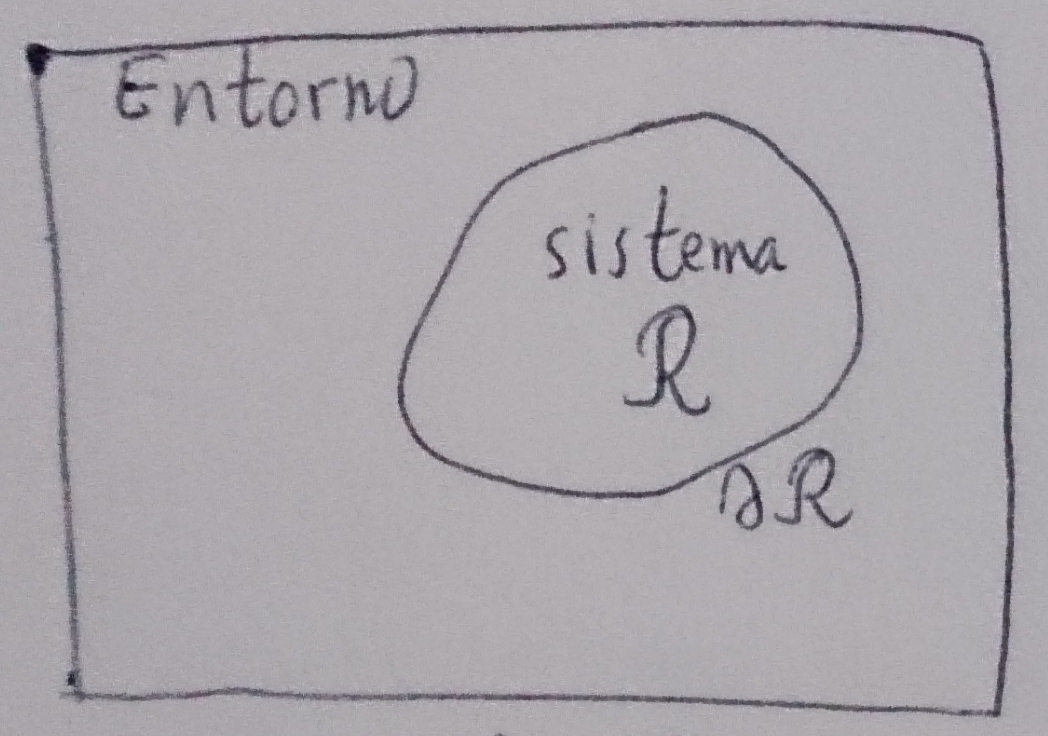
\includegraphics[width=7.6cm]{chap2_sistemaregion.JPG}
\captionof{figure}{Ilustración sencilla de un sistema que ocupa una región $\mathcal{R}$ del espacio, la frontera $\partial \mathcal{R}$, y el entorno del sistema.}\label{fig:sistemaregion}
\end{center}
\vspace{-20pt}
\end{wrapfigure}
\\ Un sistema se llama abierto si alguna región (o regiones) de la frontera permite(n) el intercambio de partículas entre el sistema y el entorno, en caso contrario, el sistema es cerrado.\\
\\
La frontera puede permitir o no la interacción del sistema con el entorno o con otro sistema. Cuando la frontera no permite interacción entre el sistema y el entorno se habla de una frontera aislante y el sistema se dice aislado. La --------- de un sistema con otro sistema o con --------- es en esencia de dos tipos para un sistema -------- a saber. interacción mecánica e interacción térmica. La interacción mecánica implica cambio del volumen (expansión o contracción) del sistema, mientras que la interacción térmica tiene asociada el concepto de calor como energía térmica que fluye entre el sistema y el entorno, en una u otra dirección sin que sea necesario un cambio de volumen ocupado por el sistema. El concepto de ca------- masa entre sistema y su entorno; las corrientes asociadas pueden extraer o dep------- calor en la región de estudio considerada.